\documentclass[12pt]{report}
\usepackage[utf8]{inputenc}
\usepackage[czech]{babel}
\usepackage{graphicx}
\graphicspath{{images/}}
\usepackage{fancyhdr}
\usepackage{makeidx}
\usepackage{natbib}
\usepackage{hyperref}
\pagestyle{fancy}
\makeindex
\makeatletter




\begin{titlepage}
\begin{center}

\Large{OSTRAVSKÁ UNIVERZITA} \\
\Large{PŘÍRODOVĚDECKÁ FAKULTA}\\
\Large{KATEDRA INFORMATIKY A POČÍTAČŮ}
\vspace{8cm}

\huge{\textbf{Tvorba mobilní aplikace}}\\
\vspace{1cm}
\Large{SEMESTRÁLNÍ PRÁCE}

\vspace{7cm}

\end{center}

\normalsize{Autor: Jan Sonnek \hfill Ostrava, 2021}

\end{titlepage}



\begin{document}


\thispagestyle{empty}

\tableofcontents
\clearpage

\chapter{STAVEBNÍ PAMÁTKY}



\section{VÍTĚZNÝ OBLOUK}



Tento 50 metrů vysoký oblouk zvaný celým jménem Arc\index{Arc} de Triomphe de l'Étoile dal postavit Napoleon Bonaparte na znak své moci a vítězství v bitvách. Byl vybudován v letech 1806 – 1836 a stojí uprostřed náměstí Charles de Gaulla na západním konci slavného pařížského bulváru Avenue des Champs-Elysées, jak můžeme vidět na obrázku ~\ref{oblouk} a ~\ref{oblouk1}. Odsud se paprskovitě rozbíhá do všech směrů dvanáct širokých tříd. Gigantický oblouk je po stranách ozdoben dvoumetrovými sochami na památku Velké armády.\cite{allen}\\
\\

\begin{figure}[h!]
\centering
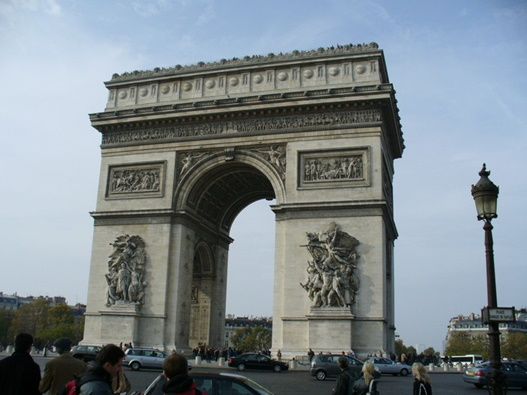
\includegraphics[scale=0.5]{images/obr1.jpg}
\caption{Vítězný oblouk 1}
\label{oblouk}

\end{figure}

V roce 1840 byl mrtvý císař přenesen během pohřebních slavností branou oblouku do Invalidovny, v roce 1885 zde byla na jednu noc vystavena rakev se zesnulým velký francouzským básníkem Victorem Hugem a 26. srpna 1944 zde oslavil francouzský národ v čele s generálem de Gaullem\index{Gaullem} osvobození.\\
\\
Pod Vítězným obloukem se nachází Památník Neznámého vojáka (Le soldat inconnu), který zde byl slavnostně pohřben 11. listopadu 1920. Oblouk od té doby slouží také jako národní pomník všech Francouzů padlých v mnoha válkách. Vyhlídková terasa skýtá velkolepý pohled na osu Louvre – Náměstí svornosti (Place de la Concorde) – La défence. Dějiny památníku dokumentuje malé Muzeum Vítězného oblouku – Musée de l'Arc de Triomphe.\cite{lacko}\\
\begin{figure}[h!]
\centering
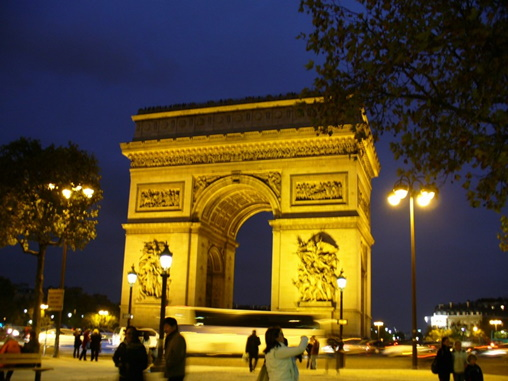
\includegraphics[scale=0.5]{images/obr2.jpg}
\caption{Vítězný oblouk 2}
\label{oblouk1}
\end{figure}
\\
Při pohledu na oblouk ze Champs-Elysées spatříte v levé spodní části reliéf zvaný Napoleonův triumf. Oslavuje vídeňskou smlouvu podepsanou v roce 1810, kdy Napoleonova říše prožívala vrcholný rozkvět. Nad Napoleonovým triumfem je umístěn reliéf líčící vítězství Napoleona nad Turky v roce 1799. Stejnou událost připomíná plátno francouzského malíře Antoina Grosa\index{Grosa}, vystavené v paláci ve Versailles. Další vítězství v bitvě je vyobrazeno na vlysu na severní straně oblouku. Přibližuje početně slabé Napoleonovo vojsko rozbíjející led na moravském rybníku. Utonuly tak tisíce nepřátelských vojáků a Francouzi zvítězili. Jeden z nejpůsobivějších reliéfů spatříte na přední části oblouku vpravo dole. Zachycuje francouzské občany odcházející bránit svůj národ před Rakušany a Prusy. Pohřeb generála Marceaua, který padl v bitvě proti rakouské armádě v roce 1796, kterou porazil pouhý rok předtím, je zvěčněn na vlysu nad reliéfem Odchodu dobrovolníků. Východní strana vlysu znázorňuje odchod francouzských vojsk o bitvy a západní jejich vítězný návrat.


\section{Eiffelova věž (Tour Eiffel)}
Asi nejznámějším monumentem Paříže vůbec je 324 metrů vysoká Eiffelova věž (obrázek ~\ref{vez1} a ~\ref{vez2}) Eiffelova postavená ze železa, přezdívaná „Železná dáma“ (La Dame de Fer). Nachází se na Champ de Mars na levém břehu řeky Seiny. Eiffelovu věž navštíví ročně přes 6 milionů návštěvníků.
\\
\begin{figure}[h!]
\centering
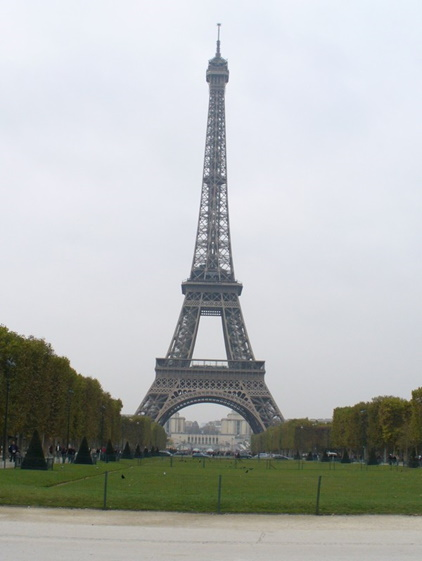
\includegraphics[scale=0.5]{images/obr3E.jpg}
\caption{Eiffelova věž}
\label{vez1}
\end{figure}
\\
\subsubsection{Kudy nahoru}
Věž je třípatrová, nahoru se dá dostat pěšky po schodech i výtahem. Schody vedou jen do druhého patra, výtahy z přízemí také do prvního a druhého patra, do třetího patra jede zase jiný výtah. Výtahy jsou celkem tři – ve východním, severním a západním pilíři.\\\\První plošina (57 m)\\
\\
Poskytuje audiovizuální muzeum ukazující stavbu a panoramatický výhled na Paříž, jsou zde restaurace.\\
\\
Druhá plošina (115 m)\\
\\
Jsou zde restaurace. Často je odtud lepší výhled než z vrcholu věže.\\
Třetí plošina (274 m)\\
\\
Dostupná jen výtahem. Je zde bar. Při dobré viditelnosti je odtud vidět i katedrála v Chartres, až na vzdálenost 65 km.\\
\\
Kromě Eiffelovy věže je krásný pohled na Paříž také od Sacré Coeur na kopci Montmartre. Pokud vás zajímá nejen pohled na Paříž, ale také na Eiffelovu věž, nejlepší pohled je od Pallais de Chaillot.
\\

\subsubsection{Historie Eiffelovy věže}
Eiffelova věž byla navržena architektem Gustavem Eiffelem (mj. autorem Sochy svobody) na počest 100. výročí Velké francouzské revoluce a Světové výstavy v roce 1889. V době vzniku byla nejvyšší stavbou světa. Původně byla věž postavena pouze na období 20 let. Mezitím získala ale svůj význam jako meteorologická stanice, proto zůstala zachována. Později se stala věž také centrem letového provozu a rozhlasového a televizního vysílání.\\
\\
Původně se věž pařížanům nelíbila, byla považována za ošklivé mostrum, architekti, spisovatelé a další umělci (Maupassant, Dumas ml., Gounod) se spojili v akci „300“ za odstranění monstra. Roku 1909 měla být věž zbourána z důvodu prošlé koncese. Počátkem 20. století se ale začala objevovat na obrazech (Pissaro, Utrillo, Seurat, Delaunay) a začali ji oslavovat i básníci (Cocteau, Apollinaire).\\\\V roce 1923 byla Antoinem Bourdellem pod Eiffelovu věž umístěna busta Eiffela, jako ocenění za jeho práci.\\

\subsubsection{Praktické informace}
\begin{itemize}
    \item Kudy na Eiffelovku: stanice metra 6 -- Passy.
    \item Vstupné: pěšky (1. a 2. patro) 3,80 €, výtah 1. patro 4,20 €, výtah 2. patro 7,70 €, výtah 3. patro 11,00 €.
    \item Nejlepší výhled: hodinu před západem slunce je nejlepší světlo.
\end{itemize}
\begin{figure}[h!]
\centering
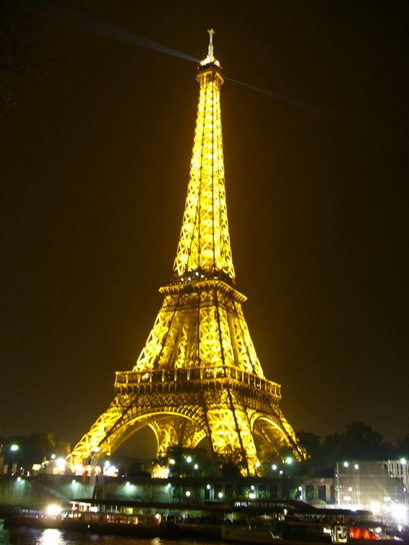
\includegraphics[scale=0.5]{images/obr4E.jpg}
\caption{Osvětlená Eiffelova věž}
\label{vez2}

\end{figure}



\chapter{KOSTELY}
\section{Sacré-Coeur}
Ačkoliv je neustále vystavována posměchu, tuto širokou daleko viditelnou baziliku připomínající šlehačkový dort si nikdo nenechá ujít. Tato bazilika postavená v novorománsko-byzantském stylu s obrovským zvonem byla v roce 1871 po prohrané válce s Německem a po porážce pařížské Komuny zamýšlena jako chrám smíření a v roce 1919 byla zasvěcena Srdci Ježíšovu. Kněží se tady dodnes ve dne v noci modlí za duše zemřelých. Na širokých schodech před vchodem lze prosedět celé hodiny a těšit se pohledu na Paříž. Interiér baziliky sice není tak impozantní jako jiné kostely ve městě, ale návštěvníky sem láká především právě panoramatická podívaná. Zvláště při západu slunce se hlouběji vryje do paměti jako jen málokterá pařížská památka.\\
\\Třpytivá mozaika Krista v byzantském stylu pochází z let 1912 – 22. vytvořil ji Luc Olivier Merson a krášlí klenbu nad kněžištěm. Vyjadřuje oddanost Francie Kristovu srdci. Nejpoutavějším prvkem interiéru je asi klenutá krypta. V jedné z kaplí je uloženo srdce Alexandra Legentila, jednoho z mecenášů Sacré-Coeur. Dveře vstupního portika dekorují nádherné bronzové reliéfy s výjevy z poslední večeře a dalšími scénami ze života Krista. Typicky vejčitá kopule baziliky je po Eiffelově veži druhou nejvyšší vyhlídkou v Paříži. Na vrchol vede točité schodiště a za jasného dne dohlédnete až do vzdálenosti 48 kilometrů. Nejvýznamnější socha v bazilice znázorňuje žehnajícího Krista. Je umístěna symbolicky v nice nad hlavním vchodem nade dvěma jezdeckými sochami.\\
\\Překrásná zvonice, kterou navrhl Lucien Magne, byla vztyčena v roce 1904 a dosahuje 80 metrů. Uvnitř je zavěšen jeden z nejtěžších zvonů na světě, devatenáctitunový La Savoyarde. Byl odlit v roce 1895 v Annecy a věnovala jej savojská diecéze. Na portiku nad hlavním vchodem se vyjímají působivé bronzové sochy francouzských světců, které odlil H. Lefébvre. Jedna představuje Janu z Arku a druhá sv. Ludvíka. Jedno z podlaží tamburu je obehnáno vitrážemi a nabízí tak úchvatný pohled na celý interiér. Architekt Paul Abadie (1875 – 1912) zakomponoval do návrhu směsici kopulí, věžiček a klasicistních prvků. Kámen ze Chateau-Landonu vylučuje, když navlhne, vápenec, který zbarvuje průčelí na bílo. Chcete-li se vyhnout výstupu do strmého kopce, využijte lanovku a cestou se kochejte pěkným výhledem. Jezdí od konce rue Foyatier poblíž place Willette\index{Willette}.

\begin{figure}[h!]
\centering
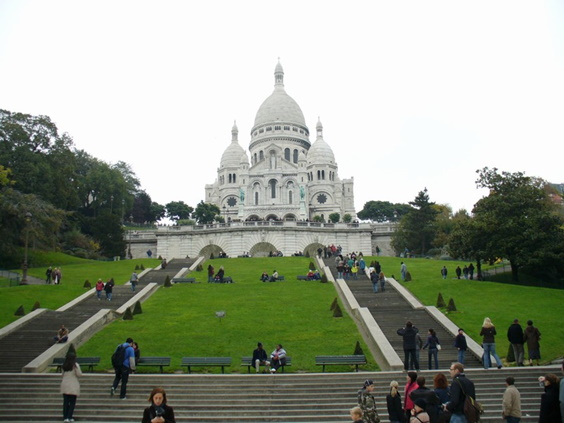
\includegraphics[scale=0.5]{images/obr5S.jpg}
\caption{Sacré-Coeur}

\end{figure}

\section{Katedrála Notre-Dame}
Tato katedrála Matky Boží je symbolem Paříže a jednou z nejvýznamnějších sakrálních staveb rané gotiky. Tady, v srdci města, kdysi stála raně křesťanská bazilika, potom románský kostel. V roce 1163 dal Maurice de Sully, biskup pařížský, zahájit stavbu, která byla dokončena v roce 1345. Od té doby byla Notre-Dame dějištěm celé řady královských slavností: v roce 1430 zde byl korunován Jindřich VI. anglickým králem Francie, v roce 1559 tu proběhla korunovace Marie\index{Marie} Stuartovny. Za Francouzské revoluce prohlásil Robespierre tuto katedrálu „chrámem rozumu“. V roce 1804 tvořila kulisu k císařské korunovaci Napleona za přítomnosti papeže. Těžké škody vzniklé v důsledku revoluce odstranil v roce 1844 Viollet-le-Duc.\cite{cada}\\
\begin{figure}[h!]
\centering
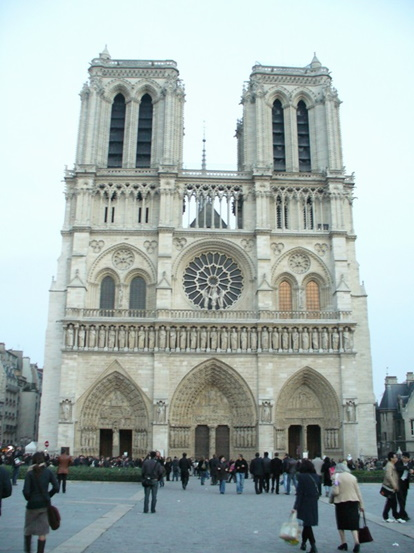
\includegraphics[scale=0.5]{images/obr6N.jpg}
\caption{Katedrála Notre-Dame}

\end{figure}\\Do katedrály lze vstoupit třemi portály s úchvatnou reliéfní výzdobou. Středověké biblické výjevy líčí život Panny Marie\index{Marie}, poslední soud a život sv. Anny. Nad nimi uvidíte galerii judských a izraelských králů. Nádherný tympanon byl ztvárněn ve 13. století a zachycuje smrt Panny Marie\index{Marie} a její slavností korunovaci v nebi. Sousoší Panny Marie\index{Marie} s dítětem na dveřním pilíři je však moderní. Slavná je dokonale krásná gotická fasáda se třemi portály a královskou galerií. Umělecky zpracovaná růžice pod arkádami Velké galerie měří v průměru deset metrů.\\\\Výhled z věže je odměnou za opravdu namáhavý výstup   věže totiž měří 69 metrů a mají 387 schodů. Návštěvníci se mohou jít podívat do té severní, v jižní je totiž zvon zvaný Emanuel vážící 13 tun. Působivý opěrný systém, podepírající východní závěr katedrály, je dílem Jeana Ravyho a má rozpětí 15 metrů. Nejlépe jej lze obdivovat z náměstí Place Jean XXIII. Mezi věžemi jsou ukryty legendární chrliče (chimiéres), jež sem umístil Viollet-le-Duc, aby odvracely zlo.\\\\Severní, jižní a západní průčelí krášlí tři skvostná rozetová okna. Vitráž\index{vitráž} s Pannou Marií obklopenou postavami ze Starého zákona z 13. století si však zachovalo pouze severní průčelí. Jižní rozetové okno vyobrazuje Krista mezi apoštoly. Více než polovina původních lavic v katedrále, které nechal zhotovit Ludvík XIV.\index{Ludvík XIV.}, se dochovala. Překrásná dřevořezba zachycuje také výjevy ze života Panny Marie\index{Marie}. U vchodu do kněžiště, naproti jihovýchodnímu pilíři transeptu, najdeme nádhernou sochu ze 14. století. Je známá jako Notre-Dame de Paris (Panna Marie\index{Marie} Pařížská) a byla sem přemístěna z kaple sv. Aignana. Sakristie uchovává staré rukopisy, relikviáře a církevní roucha. Trnová koruna a fragmenty pravého Kříže může veřejnost obdivovat vždy na Velký pátek.\cite{pecinovsky}
\begin{figure}[h!]
\centering
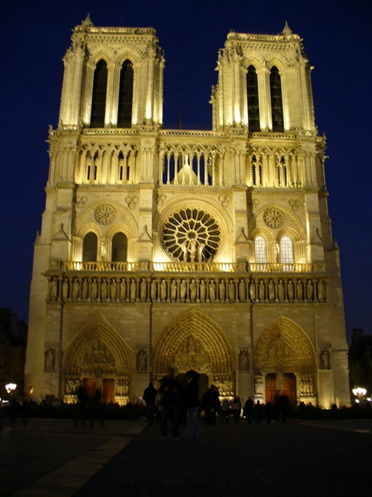
\includegraphics[scale=0.5]{images/obr7N.jpg}
\caption{Osvětlená Notre-Dame}

\end{figure}


\chapter{MUZEA}
\section{Musée du Louvre}
Louvre, jedno z nejpůsobivějších muzeí na světě, schraňuje více než 350 000 neocenitelných artefaktů. Pevnost, ve které žili králové nechal na muzeum upravit Napoleon Bonaparte.\\
\begin{figure}[h!]
\centering
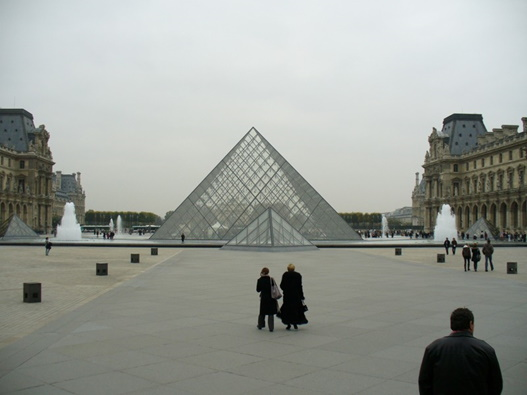
\includegraphics[scale=0.5]{images/obr8L.jpg}
\caption{Musée du Louvre}
\label{lou}
\label{Musée du Louvre}

\end{figure}
\\Hlavní vchod se nachází ve skleněné pyramidě, kterou vidíme na obrázku ~\ref{lou}, ale vejít lze i přes nákupní středisko Carrousel du Louvre v rue de Rivoli. Z haly s pokladnou vybíhají chodby do tří křídel muzea (Sully, Denon a Richelieu), obepínajících několik nádvoří\index{nádvoří}. Díla jsou rozmístěna na čtyřech podlažích a obrazy a sochy jsou uspořádány podle země původu. Uměleckým předmětům, starověkým památkám, grafikám a kresbám jsou věnována samostatná oddělení.\cite{nelson}






\subsection{Francouzské malířství}
Jedinečná kolekce pokrývá období od 14. století do roku 1848 a zahrnuje díla Georgese de La Tour, Jeana-Antoina Watteaua, Jeana-Honorého Fragonarda a dalších umělců.

\subsection{Francouzské sochařství}
K nejcennějším exponátům kolekce se řadí náhrobek\index{náhrobek} Philippa Pota od Antoina Moituriera, Koně z Marly a výtvory Pierra Pugeta na zaskleném nádvoří.

\subsection{Umění starého Egypta}
Nejlepší sbírka staroegyptského umění mimo káhirské muzeum se pyšní sfingou v kryptě, Sedícím písařem ze Sakkáry, rozměrnými sarkofágy, mumifikovanými zvířaty, hrobovými předměty a poutavými sochami zachycujícími každodenní život ve starém Egyptě.

\subsection{Umění starého Řecka}
Úchvatná kolekce umění starého Řecka obsahuje vše od kykladských sošek z 3. tisíciletí před Kristem přes antické řecké sochy z mramoru (asi 5. století př. Kr.) až po poklady z helénistického období (konec 3.-2. století př. Kr.).

\subsection{Starý Orient}
Ohromující sbírka zahrnuje mimo jiné například rekonstrukci paláce asyrského krále a rovněž zákoník\index{zákoník} krále Chammurapiho (18. století př. Kr.), nejstarší právní dokument na světě.

\subsection{Italské malířství}
Francouzská šlechta obdivovala italské umění a shromáždila značnou část zdejší sbírky (1200–1800). Mezi mnoha díly od da Vinciho uvidíte rovněž Monu Lisu, kterou můžeme vidět na obrázku ~\ref{lisa}.

\begin{figure}[h!]
\centering
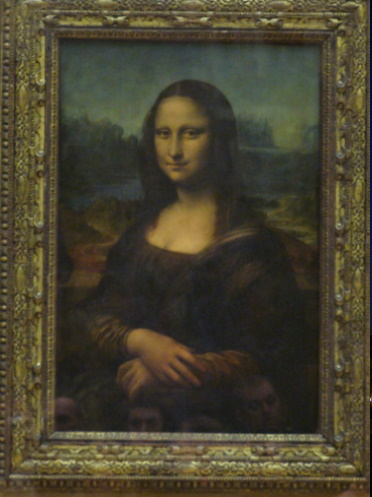
\includegraphics[scale=0.5]{images/obr9M.jpg}
\caption{Musée du Louvre}
\label{lisa}
\end{figure}


\subsection{Italské sochařství}
K nejvýznamnějším exponátům této raně renesanční sbírky náleží madona s dítětem od Donatella, která pochází z poloviny 15. století, a Michalangelovi Otroci.

\subsection{Nizozemské malířství}
Na čestném místě oddělení se vyjímají Rembrantovy práce a také výjevy z interiérů od Vermeera a podobizny od Franse Halse.

\chapter{OKOLÍ PAŘÍŽE }

\section{Versailles}
Symbol velikosti krále a vlasti a vzor snad pro každého „zámeckého architekta“ Evropy – to jsou Versailles (obrázek ~\ref{ver1}). Když se Ludvík XIV. (1638–1715) rozhodl, že přestaví malý lovecký zámeček svého otce ve Versailles 20 kilometrů západně od Paříže na nádherný palác, bylo králi Slunce právě 23 let. Francouzští panovníci sídlili v Louvru od 13. století. Od roku 1661 se Versailles staly rezidencí a sídlem vlády a absolutním mocenským centrem Francie.\\\begin{figure}[h!]
\centering
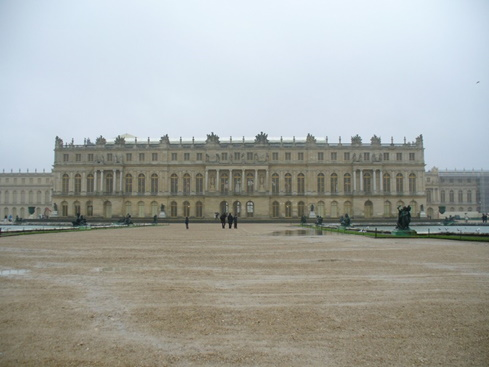
\includegraphics[scale=0.5]{images/obr10V.jpg}
\caption{Versailles}
\label{ver1}
\end{figure}\\Vše, co mohl francouzský národ nabídnout coby umělce a umělecké řemeslníky – celkem asi 30 000 lidí -, bylo posláno do Versailles, aby se podílelo na přestavbě feudálního zámku. Realizací celého díla pověřil král architekty La Vaua a Mansarta, interiérového architekta Le Bruna a zahradního architekta Le Notra. Trvalo celkem 50 let, než byl skvostný zámek dokončen tak, aby uspokojil ctižádostivost a vůli krále Slunce. Nejslavnějším a nejkrásnějším prostorem v zámeckém interiéru je Zrcadlový sál dokončený v roce 1684 a dlouhý 73 metrů. Z toho grandióuního místa dal Bismarck vyhlásit v roce 1871 Německé císařství. Uprostřed zámku je umístěna světoznámá přepychová ložnice krále. V ložnici královny, která už není tak velkolepá, přišlo na svět 19 princů a princezen.\\\\Za pozornost stojí i zahrady tohoto 680 metrů dlouhého zámku, které můžeme vidět na obrázku ~\ref{ver2}. Rozkládají se na více než 100 hektrech a musel splňovat právě tak vysoké reprezentační nároky jako sám zámek. Byly v nich vybudovány vyhlídky, široké aleje zdobené sochami a umělé kanály – „malé Benátky“. Během velkolepých barokních dvorských slavností se v parku konala operní představení. Zahradní zámek Grand Triaton, který v roce 1687 postavil Mansart, věnoval Ludvík XVI. Své manželce Marii Antoinettě. Malý zámeček Petit Trianon vznikl v roce 1762. marie Antoinetta si dala postavit i Le Hameau, vzorovou vesnici s lékárnou a mlýnem, kde se královna snažila napodobovat selský život. Za krále–občana Ludvíka Filipa v roce 1837 bylo ve Versailles zřízeno muzeum.\\\\K volné prohlídce jsou určeny Velké komnaty, Zrcadlová galerie, Galerie bitev a části obrazové galerie. Další prostory jsou přístupné jen s průvodcem.\cite{rodreguaze}

\begin{figure}[h!]
\centering
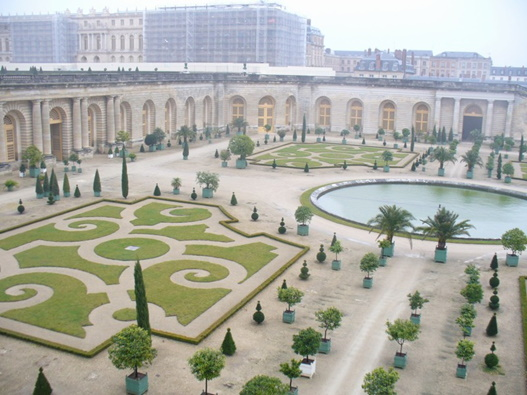
\includegraphics[scale=0.5]{images/obr11V.jpg}
\caption{Versailleský park}
\label{ver2}

\end{figure}


\listoffigures



\printindex




\begin{thebibliography}{H99}
\bibitem{allen} ALLEN, Grant, Android 4: průvodce programováním mobilních aplikací. Brno: Computer Press, 2013. 978-80-251-3782-6. 
\bibitem{cada} ČADA, Ondřej. Objektové programování: naučte se pravidla objektového myšlení. Praha: Grada, 2009. 978-80-247-2745-5.
\bibitem{lacko} LACKO, Ľuboslav. Mistrovství - Android. Brno: Computer Press., 2017. 978-80-251-4875-4.
\bibitem{pecinovsky} PECINOVSKÝ, Rudolf.  OOP a Java 8. Návrh a vývoj složitějšího projektu vyhovujícího zadanému rámci. Nakladatelství Tomáš Bruckner. Řepík-Živonín 2015. 978-80-87924-03-7.
\bibitem{nelson} NELSON, Tanner a WRIGHT Logan. Vapor Documentation [online]. [cit. 2021-03- 07]. Dostupné z: https://docs.vapor.codes
\bibitem{rodreguaze} RODREGUAZE, Sophia, Java Library: 10+ Best Libraries for Java Programmers [online]. [cit. 2021-03-07]. Dostupné z: http://noeticforce.com/useful-java-libraries
\end{thebibliography}





\end{document}
